\documentclass[14pt,a4paper]{extarticle}

\usepackage{fontspec}
\setmainfont{Times New Roman}[Ligatures=TeX]
\setmonofont{Courier New}
\newfontfamily\cyrillicfonttt{Courier New}

\usepackage{polyglossia}
\setmainlanguage{russian}
\setotherlanguage{english}

\usepackage{geometry}
\geometry{left=30mm,right=15mm,top=20mm,bottom=20mm,headheight=0pt,headsep=0pt}

\usepackage{setspace}
\onehalfspacing
\usepackage{indentfirst}
\setlength{\parindent}{1.25cm}

\usepackage{titlesec}
\titleformat{\section}{\normalsize\bfseries\centering}{\thesection.}{0.5em}{}
\titleformat{\subsection}{\normalsize\bfseries}{\thesubsection.}{0.5em}{}
\titlespacing*{\section}{0pt}{1.25em}{0.8em}
\titlespacing*{\subsection}{0pt}{1.05em}{0.55em}

\usepackage{graphicx}
\graphicspath{{figures/}}
\usepackage{caption}
\captionsetup{font=small,skip=8pt,justification=centering}
\usepackage{enumitem}
\setlist[itemize]{leftmargin=1.25cm,itemsep=0.2em,topsep=0.35em,parsep=0pt}
\setlist[enumerate]{leftmargin=1.25cm,itemsep=0.2em,topsep=0.35em,parsep=0pt}

\usepackage{pdfpages}
\usepackage{hyperref}
\hypersetup{hidelinks,unicode,pdftitle={Обзор системы выдачи кредитов банком}}

\setlength{\parskip}{0pt}
\clubpenalty=10000
\widowpenalty=10000
\emergencystretch=3em

\begin{document}

\IfFileExists{first_page.pdf}{%
\includepdf[pages=1,pagecommand={\thispagestyle{empty}}]{first_page.pdf}%
}{%
\begin{titlepage}
\thispagestyle{empty}
\begin{center}
МИНИСТЕРСТВО НАУКИ И ВЫСШЕГО ОБРАЗОВАНИЯ\\
РОССИЙСКОЙ ФЕДЕРАЦИИ

\vspace{0.8em}
ФЕДЕРАЛЬНОЕ ГОСУДАРСТВЕННОЕ АВТОНОМНОЕ\\
ОБРАЗОВАТЕЛЬНОЕ УЧРЕЖДЕНИЕ ВЫСШЕГО ОБРАЗОВАНИЯ

\vspace{0.7em}
{\bfseries НАЦИОНАЛЬНЫЙ ИССЛЕДОВАТЕЛЬСКИЙ\\ ЯДЕРНЫЙ УНИВЕРСИТЕТ «МИФИ»}

\vspace{1.6em}
Институт интеллектуальных кибернетических систем\\
Кафедра кибернетики (№~22)

\vspace{0.8em}
Направление подготовки 09.04.04\\ Программная инженерия

\vspace{1.6em}
Курсовая работа\\
по моделированию предметных сред\\
и проектированию баз данных

\vspace{1.4em}
{\bfseries «Проектирование информационной системы\\ выдачи кредитов банком»}

\vspace{0.6em}
Раздел 1. Обзор системы
\end{center}

\vspace{1.6em}
\hfill
\begin{minipage}{0.62\textwidth}
Выполнил студент группы М26-514\\
Гришанов~Н.\,В.\\[0.9em]
Преподаватель\\
Тихомирова~Д.\,В.
\end{minipage}

\vfill
\begin{center}
Москва 2026
\end{center}
\end{titlepage}
}

\renewcommand{\contentsname}{Содержание}
\tableofcontents
\newpage

\section{Обзор системы}

\subsection{Формулировка задания}

Необходимо спроектировать информационную систему выдачи кредитов банком. Система принимает заявку физического или юридического лица, проверяет заёмщика, формирует решение, готовит договор и инициирует зачисление. Исход заявки: одобрение на запрошенных условиях, одобрение на иных условиях или отказ. Он зависит от параметров заявки, кредитной истории, долговой нагрузки, обеспечения, самозапрета и правил продукта.

Ориентиры предметной области~--- два банка. Т-Банк выдаёт потребительский кредит и кредитную карту дистанционно: заявка, скоринг и подписание проходят в приложении или на сайте, деньги зачисляются на карту после периода охлаждения. Сбер совмещает удалённые каналы и офис; ипотека идёт через Домклик, кредит юридическому лицу требует проверки организации и бенефициаров.

Система хранит заёмщиков, продукты, заявки, решения, договоры, графики, обеспечение и страхование. Кредитную историю и самозапрет получает извне. Счёт зачисления и факт выдачи фиксирует сама, остаток меняет автоматизированная банковская система. Граница системы~--- путь от заявки до действующего договора с графиком и историей решений.

\subsection{Назначение и цели создания системы}

Назначение~--- выдавать кредит по одним правилам из приложения, интернет-банка и офиса. Правила скоринга, лимитов и охлаждения хранятся как данные системы, а не копируются в каждый канал.

Цели:

\begin{enumerate}
\item единый учёт заёмщиков, продуктов, заявок, решений и договоров;
\item автоматическая проверка идентификации, кредитной истории, самозапрета и долговой нагрузки;
\item поддержка кредита наличными, кредитной карты, рефинансирования, автокредита, ипотеки и кредита юридическому лицу;
\item расчёт полной стоимости кредита и индивидуальных условий договора;
\item период охлаждения только там, где он обязателен;
\item история решений, отказов и статусов;
\item отчётность по заявкам, одобрениям, отказам и выдачам.
\end{enumerate}

\subsection{Основные функциональные возможности системы}

Учёт заёмщиков. Физическое лицо: паспорт, ИНН, доход, контакты. Юридическое лицо: регистрационные сведения и выручка, связь с бенефициарами.

Учёт продуктов. Вид, валюта, границы суммы и срока, признак обеспечения и признак периода охлаждения. Продукт закрывается для новых заявок без удаления выданных договоров.

Приём заявки. Сумма, срок, канал, статус. Каналы: приложение и сайт Т-Банка; СберБанк Онлайн, Домклик, Госуслуги и офис Сбера.

Проверка самозапрета и кредитной истории. Перед потребительским кредитом запрашиваются самозапрет и кредитная история. Самозапрет устанавливается через Госуслуги с~1~марта 2025~года и через МФЦ с~1~сентября 2025~года. При действующем запрете банк отказывает. Результат хранится с заявкой.

Кредитное решение. Массовый кредит и карта закрывает скоринг, крупная сумма, расхождение данных и залог~--- андеррайтер. Хранятся результат, одобренные условия, показатель долговой нагрузки, способ принятия и причина отказа. У ипотеки решение по заёмщику и решение по объекту разделены.

Договор. Сумма, срок, ставка, полная стоимость кредита, счёт зачисления. В Т-Банке договор подписывается электронной подписью. В ипотеке Сбера выдача связана с регистрацией залога.

Период охлаждения. С~1~сентября 2025~года после подписания индивидуальных условий зачисление потребительского кредита откладывается: от~50 до~200~тысяч рублей~--- на четыре часа, свыше~200~тысяч~--- на сорок восемь часов. То же правило действует при увеличении лимита карты. В этот срок заёмщик может отказаться без процентов. Охлаждение не применяется при нескольких заёмщиках или поручителях, при залоге автомобиля с зачислением продавцу~--- юридическому лицу, при рефинансировании без роста обязательств и при ипотеке. После допустимого момента система фиксирует зачисление.

График платежей. При выдаче создаются строки: дата, основной долг, проценты, статус. Тип графика~--- аннуитетный или дифференцированный.

Обеспечение, поручительство и страхование. Залог хранит предмет и оценку. Поручитель~--- физическое лицо, возможно отличное от заёмщика. Страхование залога и добровольное страхование жизни~--- разные договоры; согласие на дополнительную услугу не является условием выдачи потребительского кредита.

Срок одобрения. Заявка закрывается отказом, истечением срока или отказом клиента, и договор при этом не создаётся. У Т-Банка на выбор условий отведено до тридцати дней, у ипотеки Сбера на поиск объекта~--- до девяноста.

Отчётность. Число заявок, доля одобрений и отказов, причины отказа, срок до выдачи, применение охлаждения, заявки с истёкшим охлаждением без зачисления.

\subsection{Конкретизация предметной области}

Предметная область~--- путь от обращения до договора с зачислением и графиком. Модель приведена на рисунке~\ref{fig:kmpo}. Прямоугольник~--- сущность, ромб~--- связь с собственными атрибутами, подпись на линии~--- имя связи. Паспорт, доход, адрес и выручка остаются атрибутами заёмщика.

\begin{figure}[p]
\centering
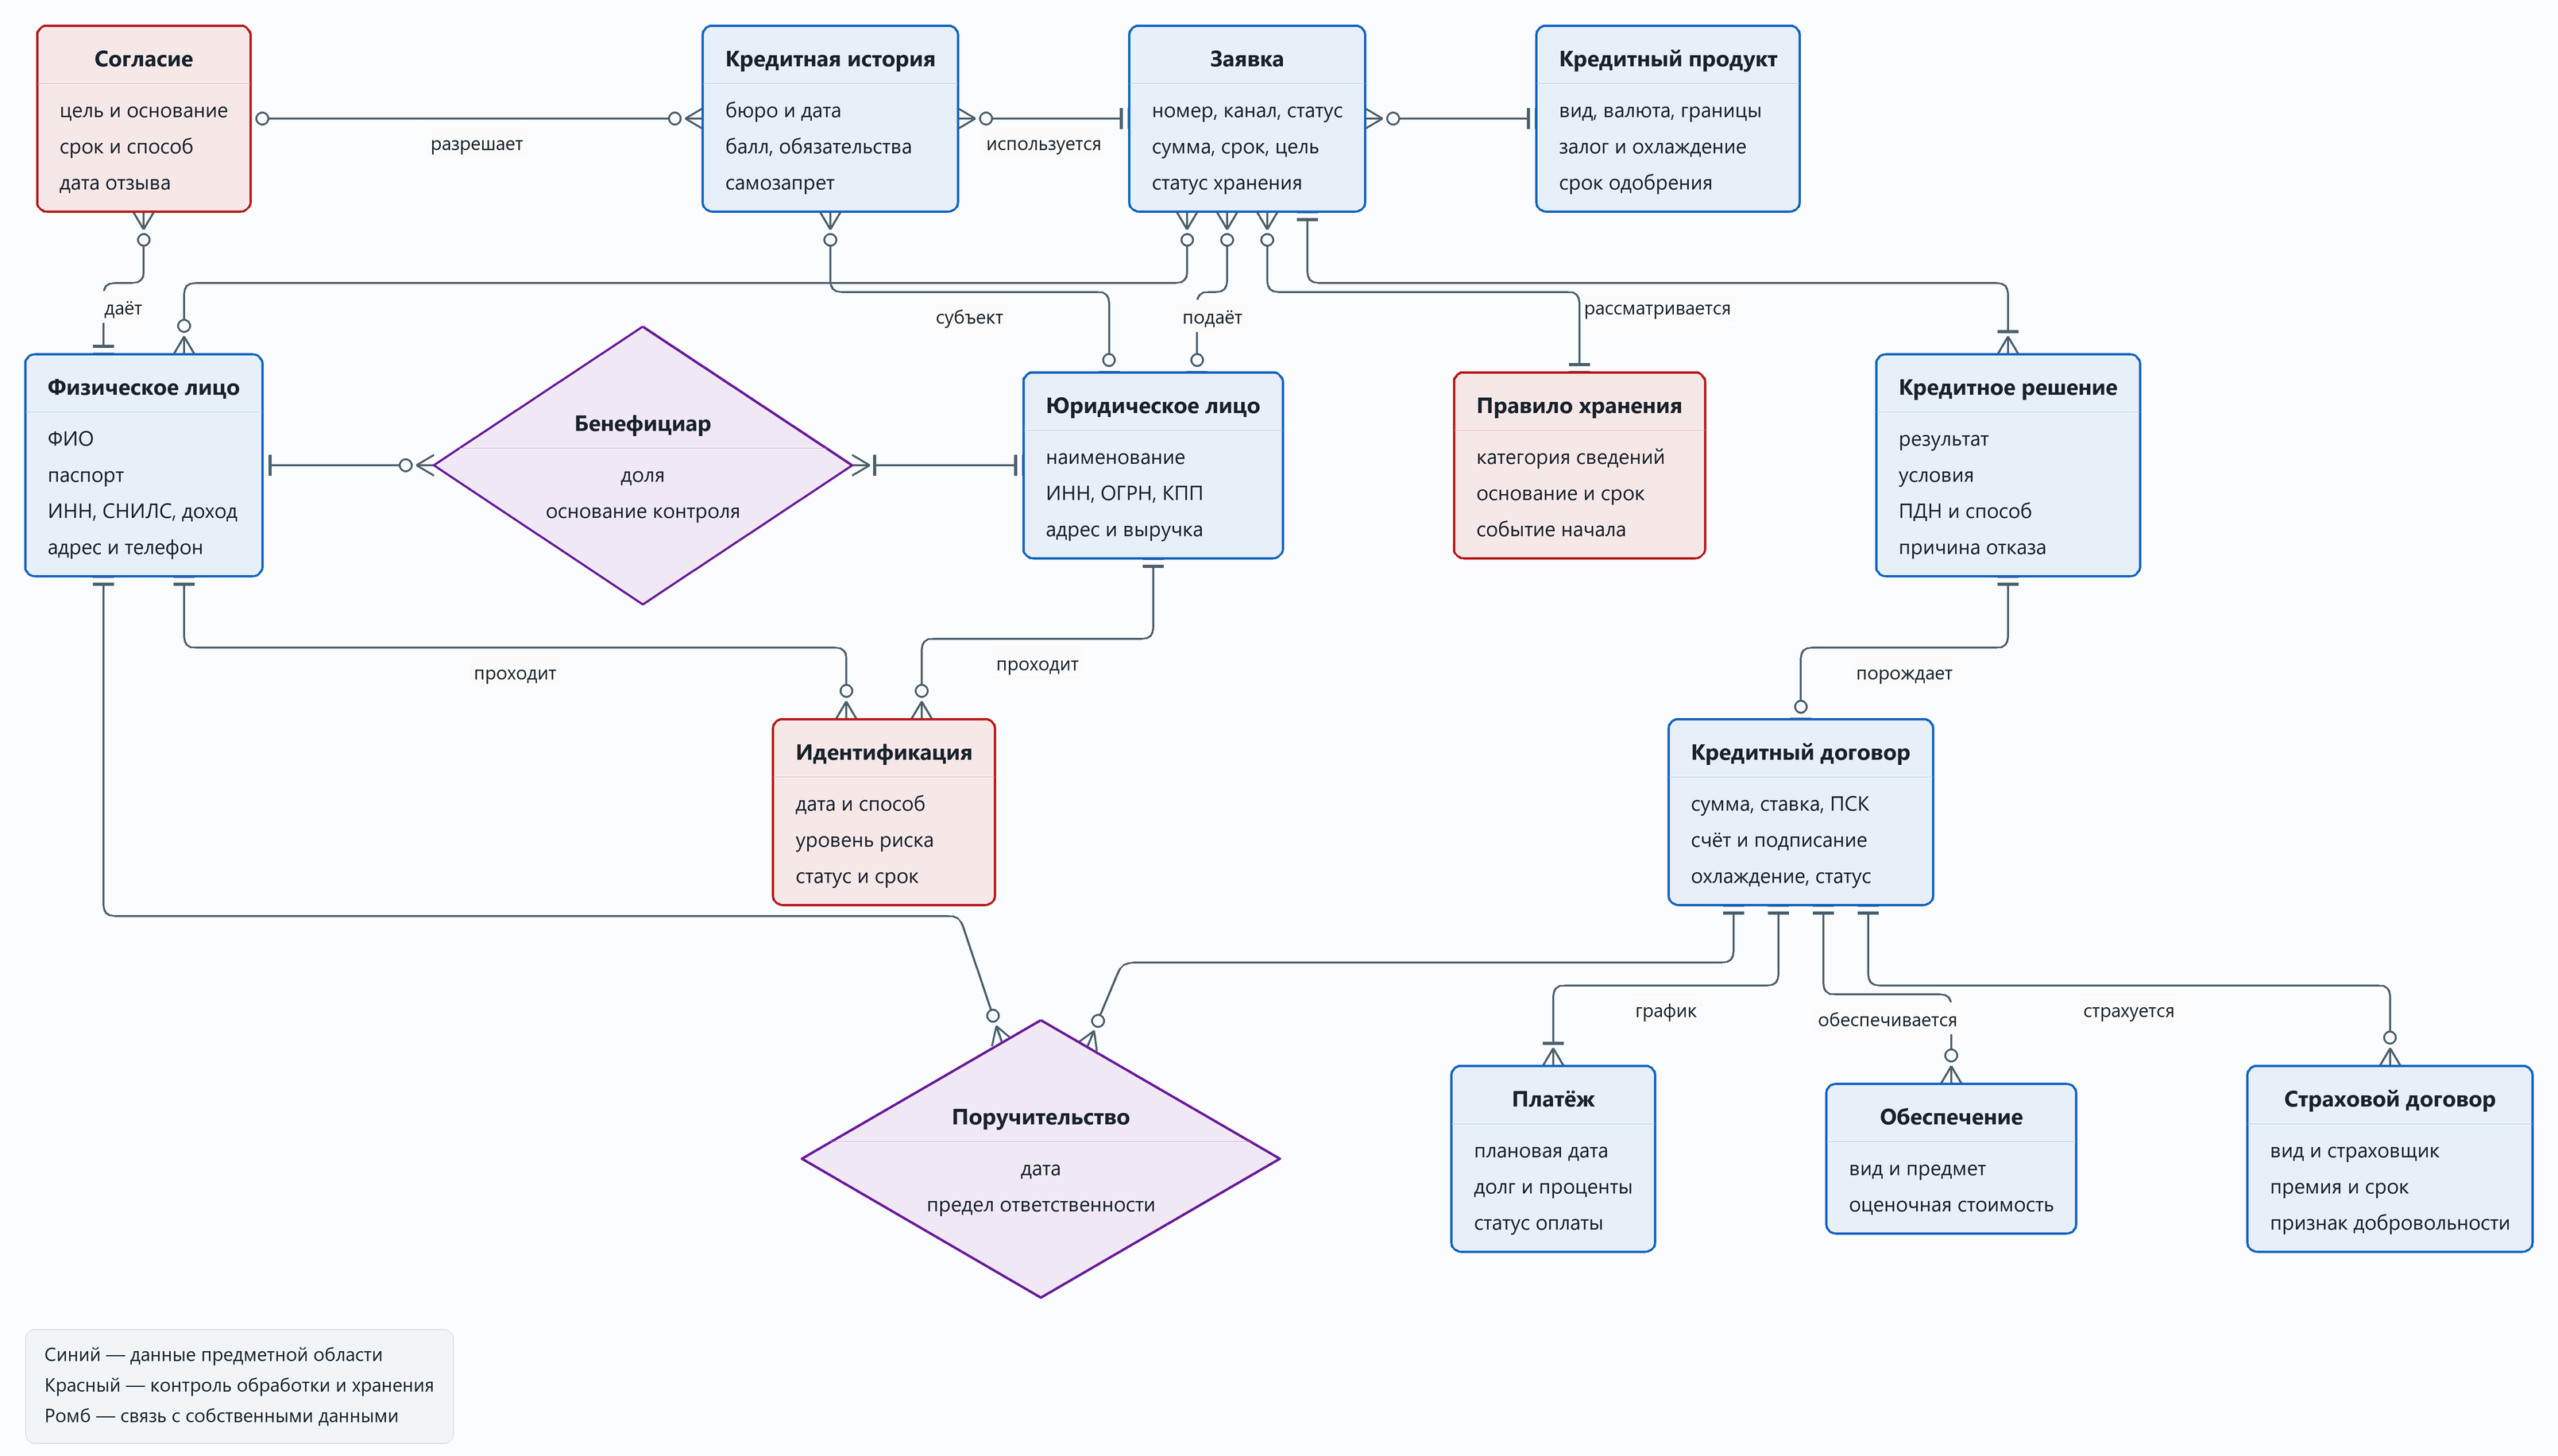
\includegraphics[width=\textwidth,height=0.9\textheight,keepaspectratio]{kmpo.png}
\caption{Концептуальная модель предметной области выдачи кредитов}
\label{fig:kmpo}
\end{figure}

Физическое лицо. Заёмщик или поручитель: ФИО, дата рождения, гражданство, паспорт, ИНН, СНИЛС, адрес, телефон, доход.

Юридическое лицо. Заёмщик-организация: наименование, ИНН, ОГРН, КПП, адрес, вид деятельности, выручка. Связано с людьми через бенефициаров.

Кредитная история. Снимок бюро под конкретную проверку: бюро, дата, балл, обязательства, самозапрет. У одного заёмщика нуль или более записей. Самозапрет заполняется только у физического лица.

Кредитный продукт. Кредит наличными, карта, рефинансирование, автокредит, ипотека, кредит юридическому лицу. Атрибуты: наименование, вид, валюта, границы суммы и срока. Один продукт~--- много заявок, заявка ссылается ровно на один продукт.

Заявка. Номер, дата, канал, сумма, срок, цель, статус. Канал: приложение, сайт, интернет-банк, офис, Домклик, представитель. Заёмщик подаёт нуль или более заявок. Статусы: черновик, на рассмотрении, одобрена, отказана, истекла, отменена клиентом, договор заключён.

Кредитное решение. Дата, результат, одобренные сумма, ставка и срок, показатель долговой нагрузки, способ принятия, причина отказа. У заявки одно или несколько решений. Одобренное решение порождает не более одного договора.

Кредитный договор. Номер, даты заключения и выдачи, сумма, ставка, срок, полная стоимость, тип графика, счёт, начало охлаждения, статус. Статусы: ожидает подписания, период охлаждения, ожидает выдачи, действует, погашен, отказ клиента до выдачи.

Платёж. Строка графика договора: плановая дата, основной долг, проценты, статус, дата оплаты. У договора один или несколько платежей.

Обеспечение. Предмет залога договора: вид, описание, идентификатор, оценка. У договора нуль или несколько предметов. Без принятого объекта ипотека не выдаётся.

Страховой договор. Вид, страховщик, премия, срок. С кредитным договором связано нуль или несколько страхований.

Бенефициар. Связь организации и физического лица: доля и основание. У организации один или несколько бенефициаров. Заёмщик и бенефициар~--- разные связи одного физического лица.

Поручительство. Связь физического лица и договора: дата и предел ответственности. Поручителей может не быть, может быть несколько. Наличие поручителя отключает период охлаждения потребительского кредита.

Кредит наличными Т-Банка на модели~--- физическое лицо, продукт без залога, автоматическое решение, договор и график, при сумме выше порога~--- охлаждение. Ипотека Сбера добавляет несколько решений, залог и страхование, без охлаждения потребительского кредита. Кредит юридическому лицу добавляет организацию, бенефициаров и решение андеррайтера.

\subsection{Пользователи системы}

Заёмщик подаёт заявку, выбирает условия в пределах лимита, подписывает договор и может отказаться до выдачи.

Кредитный специалист ведёт заявки вне одного скоринга: офисные документы, объект ипотеки, сделка, обеспечение.

Андеррайтер решает заявки, которые скоринг не закрывает: крупная сумма, расхождение данных, залог, кредит юридическому лицу. Его решение хранится отдельно от автоматического.

Администратор продуктов ведёт виды кредитов, границы сумм и сроков, признаки обеспечения и охлаждения.

Руководитель читает отчёты по заявкам, отказам и выдачам.

Администратор системы заводит сотрудников, назначает роли и ведёт справочник каналов.

\subsection{Сроки хранения информации}

Проектные сроки сверяются с документами банка и предписаниями надзора.

Идентификация клиента и сведения об операции~--- не менее пяти лет после прекращения отношений с клиентом.

Заявка, решение, договор, график, обеспечение, страхование и полученная кредитная история~--- пять лет после погашения либо после окончательного отказа.

История продукта, лимитов и правил охлаждения~--- пять лет после окончания действия редакции.

Журнал действий сотрудников~--- пять лет. Неотправленный черновик заявки~--- один год.

\subsection{События, изменяющие состояние системы}

\begin{enumerate}
\item создание или отправка заявки;
\item получение кредитной истории и результата самозапрета;
\item решение скоринга или андеррайтера;
\item одобрение на запрошенных или иных условиях, отказ банка;
\item выбор условий клиентом и подписание договора;
\item начало периода охлаждения, отказ клиента до выдачи, разрешение зачисления;
\item зачисление и построение графика;
\item регистрация обеспечения или страхования;
\item истечение одобрения без подписания, погашение договора;
\item изменение продукта или роли пользователя.
\end{enumerate}

Кредит наличными: заявка, решение скоринга, подписание, при необходимости охлаждение, зачисление и график. Отказ в периоде охлаждения закрывает договор без выдачи. Ипотека добавляет проверку объекта между решением по заёмщику и подписанием.

\subsection{Модель жизненного цикла системы}

Принята V-образная модель: требования и правила выдачи, проектирование предметной области, базы и компонентов, затем модульные, интеграционные, системные и приёмочные испытания.

Правила проверяемы до кода. Действующий самозапрет запрещает потребительский кредит. Зачисление свыше двухсот тысяч рублей раньше сорока восьми часов после подписания~--- дефект. Искусственная задержка ипотеки и рефинансирования без роста долга~--- тоже дефект. Одинаковые данные заёмщика и один продукт дают одно решение в приложении Т-Банка и в офисе Сбера.

Концептуальная модель этого раздела относится к системному проектированию. Логическая схема, запросы и физическая реализация сверяются с теми же правилами.

\subsection{Выбор инструментальных средств проектирования}

Модели системы строятся в UML Studio. Это собственная система, написанная на Python. Текст диаграммы разбирается во внутреннюю модель и раскладывается послойным алгоритмом Сугиямы: снимаются циклы, узлам назначаются уровни, порядок в ряду подбирается так, чтобы сократить пересечения, связи проводятся ортогонально. Изображение собирает библиотека Pillow.

Сам UML используется через эту систему. В ней задаются концептуальная модель предметной области, диаграммы вариантов использования и состояний заявки и договора, а также логическая и физическая модели: сущности, связи и кратности.

СУБД~--- PostgreSQL. Просмотр схемы, загрузка данных и запросы~--- DBeaver.

\end{document}
